\section{Introduction to Jolie}

Jolie is a service-oriented programming language and is built to support a
microservice architecture natively. In this section, we will introduce the
Jolie is, and show how it is used.

Jolie has a C-inspired syntax and is dynamically typed. Its interpreter is
written in Java.

The language has no native functions or methods, but instead, uses processes. A
process has no arguments and does not contain any stack. There are two
pre-defined processes, which will always be called by the interpreter, these
are called \txtl{init} and \txtl{main}.

\begin{listing}[H]
\begin{minted}{jolie}
include "console.iol"

define PrintOutput {
    println@Console(output)() // Prints 'OK'
}

init { a = 1 }

main {
    b = 2;
    c = a + b; // c = 3
    if (c == 3) {
        output = "OK"
    } else {
        output = "Bad"
    };
    PrintOutput // Calls the defined process 'PrintOutput'
}
\end{minted}
\caption{A very simple Jolie program}
\label{lst:simple_jolie}
\end{listing}

Listing \ref{lst:simple_jolie} shows a very simple application written in
Jolie.

The missing semicolons on lines 12, 14, or 16 are not mistakes. The semicolon
is not needed here, in fact, it would be a syntax error. The reason for this is
that the semicolon isn't used strictly for parsing purposes, but it instead
used for composing statements in a process.

Semicolon statements, or sequence statements, have a syntax of \joliel{A ; B}.
It should be read as: first, execute \joliel{A} then execute \joliel{B}. The
sequence statement requires both operands to be present, hence the syntax error
for adding a semicolon to the last statement of a block.

A similar composition operator is, the parallel statement, which has a syntax
of \joliel{A | B}, which reads as: execute \joliel{A} and \joliel{B} in
parallel.

These operators together allows the programmer to easily create a fork-join
workflow.  This is typically used in microservices when we want to collect data
in parallel, and continue once all of the data has been retrieved.

Jolie has different rules for scoping than most languages. In Jolie, everything
not defined in the global scope goes into the same scope. This also persists
through calls to defines. This is the reason that \verb!PrintOutput! can use
the output variable. To access the global scope we must explicitly state that
we wish to use it. Accessing a variable \joliel{a} in global scope would
require us to write \joliel{global.a}.

Several execution modes exists. The default execution mode, which was used in
Listing \ref{lst:simple_jolie}, is \joliel{single}. With an execution mode of
\joliel{single} the \joliel{main} process will run just a single time. Two
additional execution modes exist: \joliel{concurrent} and \joliel{sequential}.
Any of these two modes should be used if the Jolie program should act as a
service. When running in one of these two, the Jolie program will act as a
service.

When Jolie acts as a service, it will require the first statement of the main
procedure to be an input. An ``input'' represents an operation call (request)
going into the service, to which the Jolie program will need act upon.  Listing
\ref{lst:simple_input} shows a Jolie service being capable of answering
requests for either an operation called \joliel{echo} or \joliel{respondHello}.

\begin{listing}[H]
\begin{minted}{jolie}
main {
    [echo(request)(response) {
        response = request
    }]

    [respondHello(request)(response) {
        response = "hello"
    }]
}
\end{minted}

\caption{A simple service capable of answering requests for either of the two
    types of operations: \joliel{echo} and \joliel{respondHello}}

\label{lst:simple_input}
\end{listing}

Ports are the primitive that Jolie uses for communication, two types of ports
exist input and output. Ports describe a running service, where it is located
(\joliel{Location}), how to speak to it (\joliel{Protocol}), and finally which
operations it supports (\joliel{Interfaces}).

Listing \ref{lst:simple_port} shows an output port \joliel{Example}. This
output port will contact a web server running \joliel{http} on port 80 at
\joliel{example.com}. Only ports deal directly with protocols, this means that
the code interacting with the port remains the same, regardless of where it is
located, or which protocol it uses.

\begin{listing}[H]
\begin{minted}{jolie}
outputPort Example {
    Location: "socket://example.com:80"
    Protocol: http
    Interfaces: IExample
}
\end{minted}
\caption{A simple output port which contacts an example web server}
\label{lst:simple_port}
\end{listing}

The interface which the port uses is called \joliel{IExample}, a full
definition of it can be seen in Listing \ref{lst:simple_interface}. Two types
of operations exist in Jolie, namely \joliel{RequestResponse} and
\joliel{OneWay}.  The difference is fairly self-explanatory, the first receives
a request and returns a response, the other simply receives a request, and
produces no response. When an operation call is made from a client, and the
operation type is \joliel{RequestResponse}, then the client will wait for a
response to come back before continuing.  However, if the operation type is
\joliel{OneWay}, then the client will not wait for anything, and simply return
as soon as the message has been sent.

\begin{listing}[H]
\begin{minted}{jolie}
interface IExample {
    RequestResponse:
        anOperation(RequestType)(ResponseType)

    OneWay:
        hello(HelloType)
}
\end{minted}
\caption{An interface in Jolie defines which operations a port exposes}
\label{lst:simple_interface}
\end{listing}

Whenever the Jolie interpreter invokes an operation on an output port or
receives a request on an input port, the types will be checked. This check
ensures that incorrect requests aren't sent. It also ensures that we do not
attempt to process an incorrect request. Listing \ref{lst:simple_types} show
the request and response type of \verb!anOperation!.

\begin{listing}[H]
\begin{minted}{jolie}
type RequestType: void {
    .a: int
    .b: string
    .c: bool
    .d: double
    .e: any // any primitive type
}

type ResponseType: int {
    .aFixedArray[1, 3]: string
    .aNonFixedArray[0, *]: string
    .fieldWithChildren: void {
        .a: void {
            .b: int
        }
    }
}
\end{minted}
\caption{Jolie types are tree-like structures}
\label{lst:simple_types}
\end{listing}

In Jolie, types are tree-like structures, very similar to how, for example, XML
would be represented. Importantly the root may also contain a value, this is
different from how most other programming languages work. For example, a value
of type \joliel{ResponseType} is shown in Listing \ref{lst:value_example}.

\begin{listing}[H]
\begin{minted}{jolie}
value = 42; // root value
with (value) {
    .aFixedArray[0] = "A";
    .aFixedArray[1] = "B";
    .aNonFixedArray[0] = "foo";
    .fieldWithChildren.a.b = 1337
}
\end{minted}

\caption{An example of a value which would type-check for the type
    \joliel{ResponseType}}

\label{lst:value_example}
\end{listing}

Jolie natively supports a variety of techniques for composition of services.
The most important (for this work), which we will cover here are
\textbf{aggregation} and \textbf{embedding}.

Embedding allows for a larger service to run smaller services as inner
components. These services communicate with each other using more efficient
local communication. These embedded services can be other Jolie services, but
may also be services written in, for example, Java or even JavaScript.
Communicating with these services, through Jolie code, is done exactly the same
way as with any other service. As a result, it is entirely transparent to the
application code where the service is located.

Aggregation is a generalization of proxies and load balancers. An illustration
of this concept can be seen in Figure \ref{fig:aggregation}. Aggregation is
useful for creating a wide variety of proxy like architectural patterns. The
aggregation feature is often used alongside the courier and interface extender
features. Couriers allow the developer to insert code in-between the receiving
the request and forwarding it. These features, for example, allow you to add
authentication to a service which otherwise doesn't have it. This is done
entirely without having to touch the original service.

\begin{figure}[H]
    \centering
    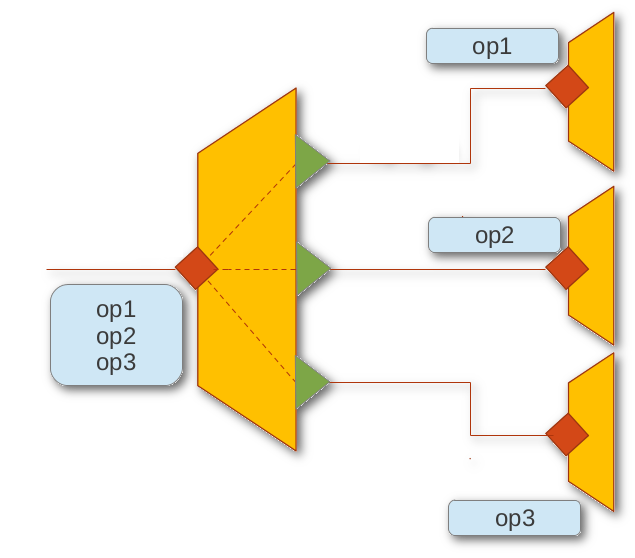
\includegraphics[width=0.6\textwidth]{pictures/aggregation.png}
    \caption{Aggregation is a generalisation of proxies and load balancers}
    \label{fig:aggregation}
\end{figure}

